\documentclass[tikz]{standalone}

\usepackage[utf8]{inputenc}
\usepackage{tikz}
\usetikzlibrary{calc,positioning,fit}
\usepackage{soul}

\begin{document}

\usetikzlibrary{arrows.meta,decorations.pathmorphing,fit,intersections,positioning,shapes.arrows,shapes.misc}

\colorlet{new}{green!50!black}

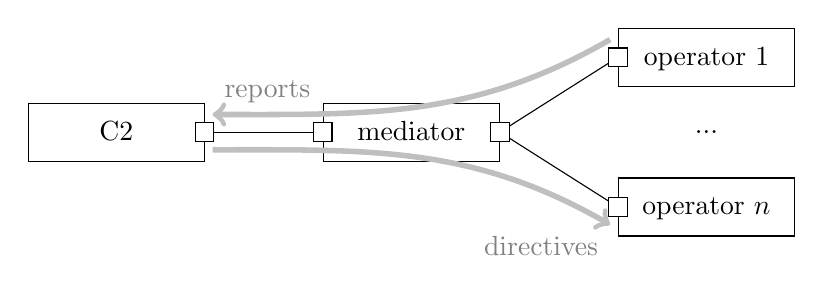
\begin{tikzpicture}
  \begin{scope}[every node/.style={rectangle,draw,text width=2cm,text height=1em,text depth=1ex,node distance=2mm and 15mm,align=center}]
    \node (master) {C2};
    \node[right=of master](med) {mediator};
    \node[above right=of med] (worker1) {operator $1$};
    \node[below right=of med] (workern) {operator $n$};
  \end{scope}
  \path (worker1) -- (workern) node[pos=.5] {...};
  \begin{scope}[every node/.style={rectangle,draw,fill=white}]
    \node (masterp) at (master.east) {};
    \node (medl) at (med.west) {};
    \node (medr) at (med.east) {};
    \node (worker1p) at (worker1.west) {};
    \node (workernp) at (workern.west) {};
  \end{scope}

  \draw (masterp.east) -- (medl.west) coordinate[pos=.5] (old);
  \draw (medr) -- (worker1p);
  \draw (medr) -- (workernp);


  % \begin{scope}[decoration={zigzag,amplitude=2mm,segment length=2mm}]
  %   \draw[orange,decorate] ([xshift=2mm]masterp.east) -- ([xshift=-2mm]medl.west);
  % \end{scope}




  \begin{scope}[color=gray!50,->,line width=2pt,every node/.style={color=gray}]
    \draw ([xshift=-1mm,yshift=1mm]worker1p.north) to[in=0,out=210] ([xshift=1mm,yshift=1mm]masterp.north) node[above right] {reports};
    \draw ([xshift=1mm,yshift=-1mm]masterp.south) to[in=150,out=0] ([xshift=-1mm,yshift=-1mm]workernp.south) node[below left] {directives};
  \end{scope}

\end{tikzpicture}





\end{document}
% Local Variables:
% mode: latex
% End:
